\documentclass[fleqn]{article}
\oddsidemargin 0.0in
\textwidth 6.0in
\thispagestyle{empty}
\usepackage{import}
\usepackage{amsmath}
\usepackage{graphicx}
\usepackage{flexisym}
\usepackage{calligra}
\usepackage{amssymb}
\usepackage{bigints} 
\usepackage[english]{babel}
\usepackage[utf8x]{inputenc}
\usepackage{float}
\usepackage[colorinlistoftodos]{todonotes}


\DeclareMathAlphabet{\mathcalligra}{T1}{calligra}{m}{n}
\DeclareFontShape{T1}{calligra}{m}{n}{<->s*[2.2]callig15}{}
\newcommand{\scriptr}{\mathcalligra{r}\,}
\newcommand{\boldscriptr}{\pmb{\mathcalligra{r}}\,}

\definecolor{hwColor}{HTML}{1a0252}

\begin{document}

  \begin{titlepage}

    \newcommand{\HRule}{\rule{\linewidth}{0.5mm}}

    \center

    \begin{center}
      
\includegraphics[height=11cm, width=11cm]{asu.png}
    \end{center}

    \vline

    \textsc{\LARGE Quantum Physics II}\\[1.5cm]

    \HRule \\[0.5cm]
    { \huge \bfseries Problem Set Five}\\[0.4cm] 
    \HRule \\[1.0cm]

    \textbf{Behnam Amiri}

    \bigbreak

    \textbf{Prof: Onur Erten}

    \bigbreak

    \textbf{{\large \today}\\[2cm]}

    \vfill

  \end{titlepage}

  \textbf{Background Information}
  \\
  \\
  \textcolor{hwColor}{
    Suppose that $S$ is a bounded region in $\mathbb{R}^3$, which has volume $V>0$, and that $f(x, y, z)$ 
    is a real-valued function, which is Riemann integrable on $S$, then the average value of $f$ on $S$ is
    $$
      \dfrac{1}{V} \bigintsss \bigintsss\limits_{S} \bigintsss f(x, y, z) ~ dV
    $$
    In Quantum mechanical calculation the expectation value is defined as
    $$
      \langle x \rangle=\bigintsss\limits_{-\infty}^{+\infty} x \psi(x, t) \psi^*(x, t) dx
    $$
    This integral can be interpreted as the average value of x that we would expect to obtain from a large number 
    of measurements. Alternatively it could be viewed as the average value of position for a large number of particles 
    which are described by the same wavefunction. For example, the expectation value of the radius of the 
    electron in the ground state of the hydrogen atom is the average value you expect to obtain from making 
    the measurement for a large number of hydrogen atoms.
    \\
    For the Hydrogen atom, we have an electron which is loacted at some distance $r$ from the origin. 
    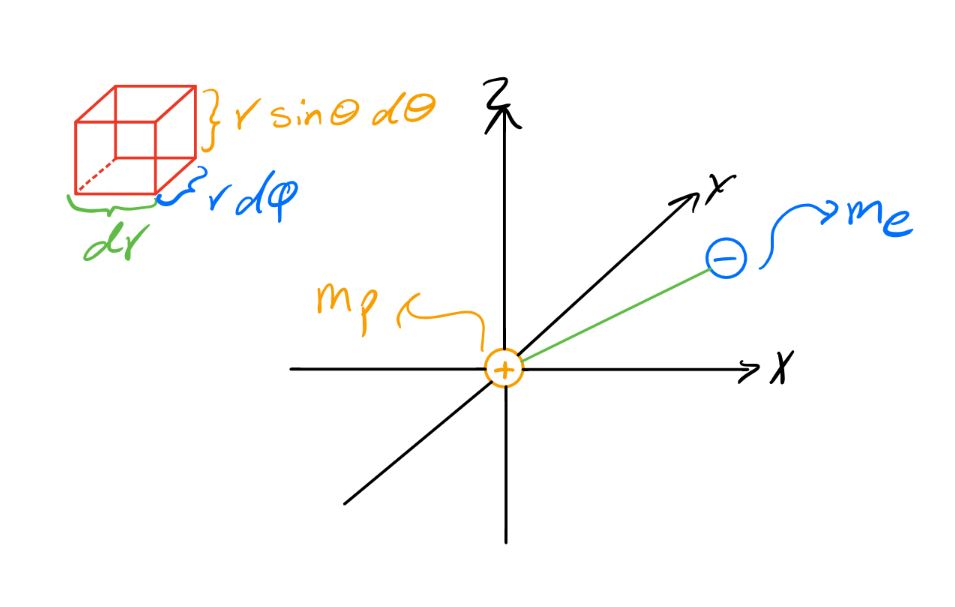
\includegraphics[height=3cm, width=5cm]{One.JPG}
    \\
    Our goal is calculating the average radius that the electron moves around. The following equation does the job for us.
    $$
      \langle W \rangle=\bigintsss\limits_{0}^{2\pi} d\phi 
      ~ \bigintsss\limits_{0}^{\pi} sin(\theta) d\theta 
      ~ \bigintsss\limits_{0}^{\infty} r^2 dr ~ W \psi^*(r, \theta, \phi) \psi(r, \theta, \phi) 
    $$
    Given that the hydrogen atom contains a nucleus and an electron, quantum mechanics allows one to predict the probability of finding the electron at 
    any given radial distance $r$. It is given by the square of a mathematical function known as the \emph{wavefunction} which is a 
    solution of the Schr$\ddot{o}$dinger equation. The lowest energy equilibrium state of the hydrogen atom is known as the ground state.
    \\
    Page 148 of the textbook states the ground state of hydrogen as $\psi_{1, 0, 0}(r, \theta, \phi)=\dfrac{1}{\sqrt{\pi a^3}} e^{-r/a}$
    where $a=\dfrac{4 \pi \epsilon_0 \hbar^2}{m_e e^2}$ is the Bohr radius.
    \\
  } 

  \begin{enumerate}
    \item \textbf{4-15}
    \begin{enumerate}
      \item Find $\langle r \rangle$ and $\langle r^2 \rangle$ for an electron in the ground state of hydrogen. Express your
      answers in terms of the Bohr radius. 

        \textcolor{hwColor}{
          \\
          $
            \langle r \rangle=\bigints\limits_{0}^{2\pi} 
            ~ \bigints\limits_{0}^{\pi} 
            ~ \bigints\limits_{0}^{\infty} ~ r ~ \psi^*_{100} \psi_{100} ~ r^2 sin(\theta) dr ~ d\theta ~ d\phi
            \\
            \\
            \\
            =\bigints\limits_{0}^{2\pi} d\phi
            ~ \bigints\limits_{0}^{\pi} sin(\theta) d\theta 
            ~ \bigints\limits_{0}^{\infty} r^3 ~ \dfrac{1}{\sqrt{\pi a^3}} e^{-r/a} ~ \dfrac{1}{\sqrt{\pi a^3}} e^{-r/a} dr
            \\
            \\
            \\
            =\left(2 \pi\right).\left(2\right).\dfrac{1}{\pi a^3} \bigints\limits_{0}^{\infty} r^3 e^{-2r/a} ~ dr
            \\
            \\
            \\
            =\left(2 \pi\right).\left(2\right).\left(\dfrac{1}{\pi a^3} \dfrac{3!}{(2/a)^{3+1}}\right)
            \\
            \\
            \\
            \therefore ~~~ \langle r \rangle=\dfrac{3}{2}a ~~~~~ \checkmark
            \\
            \\
            \\
            \\
            \\
            \langle r^2 \rangle=\bigints\limits_{0}^{2\pi} 
            ~ \bigints\limits_{0}^{\pi} 
            ~ \bigints\limits_{0}^{\infty} ~ r^2 ~ \psi^*_{100} \psi_{100} ~ r^2 sin(\theta) dr ~ d\theta ~ d\phi
            \\
            \\
            \\
            =\bigints\limits_{0}^{2\pi} d\phi
            ~ \bigints\limits_{0}^{\pi} sin(\theta) d\theta 
            ~ \bigints\limits_{0}^{\infty} r^4 ~ \dfrac{1}{\sqrt{\pi a^3}} e^{-r/a} ~ \dfrac{1}{\sqrt{\pi a^3}} e^{-r/a} dr
            \\
            \\
            \\
            =\left(2 \pi\right).\left(2\right).\dfrac{1}{\pi a^3} \bigints\limits_{0}^{\infty} r^4 e^{-2r/a} ~ dr
            \\
            \\
            \\
            =\left(2 \pi\right).\left(2\right).\left(\dfrac{1}{\pi a^3} \dfrac{4!}{(2/a)^{4+1}}\right)
            \\
            \\
            \\
            \therefore ~~~ \langle r^2 \rangle=3a^2 ~~~~~ \checkmark
          $
        }

      \pagebreak

      \item Find $\langle x \rangle$ and $\langle x^2 \rangle$ for an electron in the ground state of hydrogen. 
      \emph{Hint: This requires no new integration-note that $r^2=x^2+y^2+z^2$, and exploit the symmetry of the ground state}

        % \textcolor{hwColor}{

        % }


      \item Find $\langle x^2 \rangle$ in the state $n=2$, $\ell$, $m=1$. \emph{Hint: this state is not symmetrical in 
      $x, y,z.$ Use $x=r sin(\theta) cos(\phi)$.}

        % \textcolor{hwColor}{

        % }


    \end{enumerate}

    \item \textbf{4-15} What is the \emph{most probable} value of $r$, in the ground state of hydrogen? 
    (The answer is \emph{not zero!}) \emph{Hint:} First you must figure out the probablity that the electron would be found between
    $r$ and $r+dr$.

      % \textcolor{hwColor}{

      % }


  \end{enumerate}

\end{document}